\documentclass{beamer}
\usetheme{jmct}          % vendored in theme/; \usetheme[titlesize=48]{jmct} for long titles

\usepackage{amsmath,amssymb}
\usepackage{booktabs}
\usepackage{animate}

% Charts are built by `make` from plots/*.tex into build/plots/;
% your own images go in figs/.
\graphicspath{{build/plots/}{figs/}}

\usetikzlibrary{positioning,arrows.meta,calc,decorations.pathreplacing,shapes.geometric,shapes.callouts}

% TikZ styles in the theme palette (colours come from the jmct theme).
\tikzset{
  >={Stealth[length=6pt]},
  box/.style={draw=dark-lucid-blue, line width=0.8pt, rounded corners=2pt,
              fill=white, text=dark-gray, minimum height=0.9cm,
              minimum width=2cm, align=center, font=\small},
  hot/.style={box, draw=my-magenta, text=my-magenta},
  dot/.style={circle, draw=dark-lucid-blue, line width=0.8pt, fill=white,
              text=dark-gray, minimum size=0.8cm, font=\small},
  link/.style={->, draw=dark-gray, line width=0.7pt},
  note/.style={text=light-gray, font=\footnotesize},
  % Overlays inside a tikzpicture: \node[visible on=<2->] ...
  % The node keeps its space while hidden, so the picture never jumps.
  invisible/.style={opacity=0, text opacity=0},
  visible on/.style={alt={#1{}{invisible}}},
  alt/.code args={<#1>#2#3}{\alt<#1>{\pgfkeysalso{#2}}{\pgfkeysalso{#3}}},
}

% A part divider: the part name, large, on an otherwise empty frame.
% \partslide is just the frame body, so a divider can carry overlays
% (e.g. \correction below) while \partframe adds the \section entry.
% Optional first argument: a subtitle line underneath, in the subtitle font and
% the title colour (beamer colour `title`, i.e. dark-gray):
%   \partframe[An optional subtitle]{Part name}
\newcommand{\partslide}[2][]{%
  \vfill\centering{\usebeamerfont{title}\fontsize{40}{44}\selectfont #2\par}%
  \if\relax\detokenize{#1}\relax\else
    \vskip 0.8em{\usebeamerfont{subtitle}\usebeamercolor[fg]{title}#1\par}%
  \fi
  \vfill}
\newcommand{\partframe}[2][]{%
  \section{#2}%
  \frame{\partslide[#1]{#2}}%
}

% \correction{old}{new}: typeset `old' exactly as plain text would (a TikZ node
% with zero padding, sitting on the baseline), then from overlay 2 on, strike
% it out and write `new' above it like a pen correction on paper.  Both marks
% are `overlay', so they take no space and nothing else on the slide moves.
\colorlet{correction-ink}{galois-blue}
\newcommand{\correction}[2]{%
  \tikz[baseline=(old.base)]{%
    \node[inner sep=0pt, outer sep=0pt] (old) {#1};%
    \onslide<2->{%
      \draw[overlay, correction-ink, line width=2.2pt, line cap=round]
        ([xshift=-4pt, yshift=-4pt]old.west) -- ([xshift=4pt, yshift=2pt]old.east);%
      \node[overlay, correction-ink, anchor=south, rotate=4, inner sep=0pt,
            font=\itshape] at ([yshift=6pt]old.north) {#2};%
    }%
  }%
}

% A frame holding one chart, scaled to fit under the frame title.
\newcommand{\chartframe}[2]{%
  \frame{\frametitle{#1}%
    \centering\includegraphics[width=\textwidth,height=0.8\textheight,keepaspectratio]{#2}}%
}

\title{Probity}
\subtitle{Jos\'e Manuel Calder\'on Trilla \\
          Harrison Goldstein}
\date{}

\begin{document}

\frame{\titlepage}

%%%%%%%%%%%%%%%%%%%%%%%%%%%%%%%%%%%%%%%%
%%% Text
%%%%%%%%%%%%%%%%%%%%%%%%%%%%%%%%%%%%%%%%

% One frame, two slides: plain on the first, the pen correction on the second.
\section{Formal Methods is Ascendant}
\frame{\partslide{Formal \correction{Methods}{Slop} is Ascendant}}

\chartframe{Lean: 9 years to 2.4M lines, then 13.5M in 11 days}{leanloc}
\chartframe{Interest in Lean and software verification is climbing}{trends}

\frame{
  \frametitle{Common forms of formal methods slop}
  \begin{itemize}
    \item<2-2> Agents change your properties in order to meet the code
    \item<3-3> Agents prove that your code meets the specification defined
              \blueite{by your code}, which is vacuously true
    \item<4-4> The property or theorem as stated is subtly (but importantly)
              different from what you asked for: an \blueit{interpretability
              problem} for specifications
    \item<5-5> Little to no thought given to the link between \blueit{the model}
              and \blueit{the actual implementation}
    \item<6-6> Bad PBT generators
  \end{itemize}
}

\frame{
  \frametitle{Claude, make me a verified Minecraft in Lean}
  \centering
  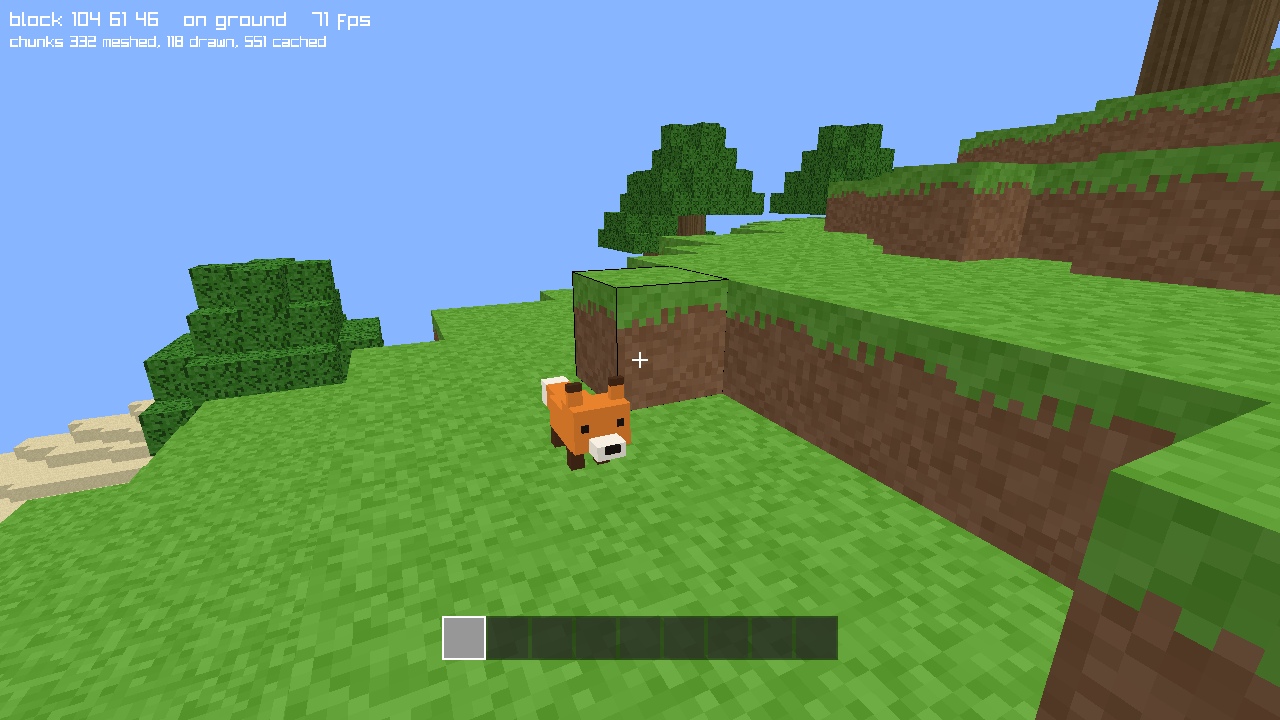
\includegraphics[width=\textwidth]{fox}
  Works, sure, but Lean was happy to use a C-library without thinking about how that library should behave!
}


\frame{
  \frametitle{Why us?}
  \begin{columns}
    \begin{column}{.5\textwidth}
      Jos\'e
      \begin{itemize}
        \item<2-> \blueit{Formal Methods @ Galois}
        \item<3-> \blueit{Faculty @ University of Maryland}
        \item<4-> \blueit{Non-profit experience as Exec. Dir. of the Haskell Foundation}
        \item<5-> \blueit{Formal Methods consultant helping Co.s leverage these tools}
      \end{itemize}
    \end{column}
    \begin{column}{.5\textwidth}
      Harry
      \begin{itemize}
        \item<2-> \blueit{Studied engineering leadserhip @ Cornell}
        \item<3-> \blueit{PLT and Property-based testing \@ UPenn}
        \item<4-> \blueit{User studies on developers using semi-formal methods}
        \item<5-> \blueit{Current research on interperability of specifications}
      \end{itemize}
    \end{column}
  \end{columns}
}

%% Any frame containing a codeblock needs [fragile].
%\begin{frame}[fragile]
%  \frametitle{A code frame}
%  \begin{codeblock}[language=Python]
%def placeholder(xs):
%    # replace me
%    return sum(x * x for x in xs)
%  \end{codeblock}
%\end{frame}
%
%\frame{
%  \frametitle{A quote}
%  \myquote{A quotation goes here, long enough to wrap onto a second
%    line so the layout is visible.}{Someone}{Year}
%}

%%%%%%%%%%%%%%%%%%%%%%%%%%%%%%%%%%%%%%%%
%%% Charts (pgfplots, built from plots/*.tex)
%%%%%%%%%%%%%%%%%%%%%%%%%%%%%%%%%%%%%%%%

%\partframe{Charts}

%\frame{
%  \frametitle{Two charts side by side}
%  \begin{columns}[T]
%    \column{0.5\textwidth}
%      \centering\includegraphics[width=\linewidth]{line}\\[4pt]
%      \footnotesize Left caption
%    \column{0.5\textwidth}
%      \centering\includegraphics[width=\linewidth]{histogram}\\[4pt]
%      \footnotesize Right caption
%  \end{columns}
%}

%%%%%%%%%%%%%%%%%%%%%%%%%%%%%%%%%%%%%%%%
%%% Diagrams (TikZ, inline so overlays work)
%%%%%%%%%%%%%%%%%%%%%%%%%%%%%%%%%%%%%%%%

%\partframe{Diagrams}

%% A pipeline revealed one stage per step.
%\frame{
%  \frametitle{A pipeline, step by step}
%  \centering
%  \begin{tikzpicture}[node distance=1.1cm]
%    \node[box]                                  (a) {Stage A};
%    \node[box, right=of a, visible on=<2->]     (b) {Stage B};
%    \node[box, right=of b, visible on=<3->]     (c) {Stage C};
%    \node[hot, below=1.2cm of b, visible on=<4->] (d) {Feedback};
%
%    \draw[link, visible on=<2->] (a) -- (b);
%    \draw[link, visible on=<3->] (b) -- (c);
%    \draw[link, visible on=<4->] (c.south) |- (d.east);
%    \draw[link, visible on=<4->] (d.west) -| (a.south);
%
%    \node[note, above=0.2cm of a]                  {input};
%    \node[note, above=0.2cm of c, visible on=<3->] {output};
%  \end{tikzpicture}
%}
%
%% A small graph; nodes placed by hand, edges by name.
%\frame{
%  \frametitle{A graph}
%  \centering
%  \begin{tikzpicture}[x=2.2cm, y=1.5cm]
%    \node[dot] (r)  at (0,0)    {r};
%    \node[dot] (a)  at (-1,-1)  {a};
%    \node[dot] (b)  at (1,-1)   {b};
%    \node[dot] (c)  at (-1.5,-2) {c};
%    \node[dot] (d)  at (-0.5,-2) {d};
%    \node[dot, draw=my-magenta, text=my-magenta] (e) at (1,-2) {e};
%
%    \foreach \u/\v in {r/a, r/b, a/c, a/d, b/e}
%      \draw[link] (\u) -- (\v);
%    \draw[link, my-magenta, dashed] (e.east) to[out=30, in=0, looseness=1.2] (r.east);
%    \node[note, below=0.15cm of e] {a highlighted node};
%  \end{tikzpicture}
%}
%
%% A layered stack; fit draws a bracket around a group of layers.
%\frame{
%  \frametitle{A layered stack}
%  \centering
%  \begin{tikzpicture}[layer/.style={box, minimum width=6cm}, node distance=0.15cm]
%    \node[layer]                 (l1) {Layer one};
%    \node[layer, below=of l1]    (l2) {Layer two};
%    \node[hot, minimum width=6cm, below=of l2] (l3) {Layer three};
%    \node[layer, below=of l3]    (l4) {Layer four};
%
%    \draw[decorate, decoration={brace, amplitude=6pt}, dark-lucid-blue, line width=0.8pt]
%      ($(l1.north east)+(0.2,0)$) -- ($(l2.south east)+(0.2,0)$)
%      node[midway, right=8pt, text=dark-gray, font=\small] {a group};
%  \end{tikzpicture}
%}

%%%%%%%%%%%%%%%%%%%%%%%%%%%%%%%%%%%%%%%%
%%% End
%%%%%%%%%%%%%%%%%%%%%%%%%%%%%%%%%%%%%%%%

% Tech transfer, today vs. with Probity.  Overlay 1: today; overlay 2 adds Probity.
%%%%%%%%%%%%%%%%%%%%%%%%%%%%%%%%%%%%%%%%
%%% Probity
%%%%%%%%%%%%%%%%%%%%%%%%%%%%%%%%%%%%%%%%

\partframe[Formal Methods, honestly.]{Probity}

% The toolbox as a pyramid: current SWE practice at the base, Embedding at the
% peak, and a brace leaning on the right slope.
%
% Switch: \buildpyramidtrue reveals the pyramid one slice per click and the
% brace on the click after; \buildpyramidfalse shows everything at once.
\newif\ifbuildpyramid
\buildpyramidfalse
%
% \toolpyramid{<y where the brace starts>}{<brace label>}
%   0.75 = bottom of Property-based testing; 0 = bottom of the whole pyramid.
\newcommand{\toolpyramid}[2]{%
  \begin{tikzpicture}
    % base width \B, total height \H; the half-width shrinks linearly with height.
    % Five slices of 0.75cm, then a taller peak so its label fits.
    \def\B{8.4}\def\H{4.95}
    \foreach \i/\ya/\yb/\name/\fillc/\txt in {
        0/0.00/0.75/{Current SWE practice}/{light-gray!40}/{\bfseries},
        1/0.75/1.50/{Property-based testing}/{dark-lucid-blue!12}/{},
        2/1.50/2.25/{Semantics}/{dark-lucid-blue!20}/{},
        3/2.25/3.00/{Specifications}/{dark-lucid-blue!28}/{},
        4/3.00/3.75/{Modeling}/{dark-lucid-blue!36}/{},
        5/3.75/4.95/{Embedding}/{dark-lucid-blue!44}/{}} {
      \ifbuildpyramid\pgfmathtruncatemacro{\s}{\i+2}\else\def\s{1}\fi
      \pgfmathsetmacro{\wa}{\B/2*(1-\ya/\H)}
      \pgfmathsetmacro{\wb}{\B/2*(1-\yb/\H)}
      \begin{scope}[visible on=<\s->]
        \filldraw[fill=\fillc, draw=off-white, line width=1.6pt, line join=round]
          (-\wa,\ya) -- (\wa,\ya) -- (\wb,\yb) -- (-\wb,\yb) -- cycle;
        \node[font=\footnotesize\txt, text=dark-gray, anchor=base]
          at (0,{\ya+(\i==5 ? 0.13 : 0.2)}) {\name};
      \end{scope}
    }
    % Brace leaning on the right slope, from height #1 up to the peak,
    % offset 0.22cm outward (perpendicular to the edge).
    \ifbuildpyramid\def\bs{8}\else\def\bs{1}\fi
    \pgfmathsetmacro{\wbot}{\B/2*(1-#1/\H)}
    \coordinate (peak) at (0,\H);
    \coordinate (foot) at (\wbot,#1);
    \coordinate (bt) at ($(peak)!0.22cm!90:(foot)$);
    \coordinate (bb) at ($(foot)!0.22cm!-90:(peak)$);
    \begin{scope}[visible on=<\bs->]
      \draw[decorate, decoration={brace, amplitude=7pt}, my-magenta, line width=1pt]
        (bt) -- (bb);
      \node[anchor=south west, align=left, font=\small\bfseries, text=my-magenta, inner sep=0pt]
        at ($($(bt)!0.5!(bb)$)!16pt!90:(bb)$) {#2};
    \end{scope}
    % fixed right edge, so the pyramid sits in the same place whatever the label
    \path (6.3,0);
  \end{tikzpicture}%
}

\frame{
  \frametitle{A pathway from today's practice to formal methods}
  Help engineers \blueite{understand the toolbox}:
  \vfill
  \centering
  \toolpyramid{0.75}{Can all be\\done in Lean}
  \vfill
}

% Same pyramid; now the brace covers the base too.
\frame{
  \frametitle{A pathway from today's practice to formal methods}
  Help engineers \blueite{understand the toolbox}:
  \vfill
  \centering
  \toolpyramid{0}{Soon it will\\all be done in\\formal languages}
  \vfill
}



\frame{
  \frametitle{Research tools ready for SWE \emph{and} agent use}
  \begin{itemize}
    \item<2-2> \blueit{Scaffolding} for common formal-methods tasks
    \item<3-3> \blueit{User studies}
    \item<4-4> \blueit{Maintaining} formal-methods tools that are important,
              but not interesting to PhDs, e.g.:
      \begin{itemize}
        \item Lean WASM backend
        \item KLEE on modern LLVM
        \item Microsoft Code Contracts (RIP)
        \item Contributing to QuickChick for Lean
      \end{itemize}
  \end{itemize}
}

\frame{
  \frametitle{Tech transfer, today and with Probity}
  \centering
  \begin{tikzpicture}[
      x=1cm, y=1cm,
      lbl/.style={font=\scriptsize, text=dark-gray, align=center},
      rowlbl/.style={font=\small\bfseries, text=my-magenta, anchor=west},
      flow/.style={->, draw=dark-gray, line width=0.9pt},
      spiky/.style={star, star points=11, star point ratio=2.2, minimum size=1.15cm,
                    inner sep=0pt, fill=my-magenta!85, draw=my-magenta, line width=0.6pt,
                    % centre hole, like the gear, so it reads as the same object
                    path picture={\filldraw[fill=off-white, draw=my-magenta, line width=0.6pt]
                      (path picture bounding box.center) circle (0.12);}},
      % the smoothed artifact: a gear (10 rounded teeth, centre hole)
      gear/.pic={
        \fill[my-magenta!85, draw=my-magenta, line width=0.6pt, even odd rule,
              rounded corners=0.9pt]
          (0:0.36) \foreach \i in {0,...,9} {
            -- (\i*36+5:0.36) -- (\i*36+9:0.52) -- (\i*36+23:0.52) -- (\i*36+27:0.36)
            -- (\i*36+36:0.36) } -- cycle
          (0,0) circle (0.13);
      },
      bubble/.style={rectangle callout, rounded corners=3pt, fill=white, draw=dark-gray,
                     line width=0.6pt, font=\scriptsize\itshape, text=dark-gray,
                     inner sep=4pt, align=center},
      flask/.pic={
        \fill[lucid-blue!70] (-0.29,-0.15) -- (-0.4,-0.35) -- (0.4,-0.35) -- (0.29,-0.15) -- cycle;
        \draw[dark-gray, line width=0.9pt, line join=round]
          (-0.12,0.4) -- (-0.12,0.15) -- (-0.4,-0.35) -- (0.4,-0.35) -- (0.12,0.15) -- (0.12,0.4);
        \draw[dark-gray, line width=0.9pt] (-0.18,0.4) -- (0.18,0.4);
        \fill[white] (-0.08,-0.25) circle (0.035) (0.1,-0.2) circle (0.025);
      },
      % a cartoon person; #1 = mouth (frown or smile)
      person/.pic={
        \draw[dark-gray, line width=0.9pt, fill=white] (0,0.42) circle (0.17);
        \fill[dark-gray] (-0.06,0.46) circle (0.018) (0.06,0.46) circle (0.018);
        \draw[dark-gray, line width=0.9pt, line cap=round]
          (0,0.25) -- (0,-0.12)            % body
          (-0.22,0.12) -- (0,0.18) -- (0.22,0.12)  % arms
          (0,-0.12) -- (-0.14,-0.42)       % legs
          (0,-0.12) -- (0.14,-0.42);
      },
      frown/.pic={\draw[dark-gray, line width=0.7pt] (-0.06,0.35) arc[start angle=150, end angle=30, radius=0.07];},
      smile/.pic={\draw[dark-gray, line width=0.7pt] (-0.06,0.39) arc[start angle=210, end angle=330, radius=0.07];},
      docs/.pic={
        \foreach \d in {0.12,0.06,0} {
          \draw[dark-gray, line width=0.7pt, fill=white] (-0.22+\d,-0.28+\d) rectangle (0.22+\d,0.28+\d);
        }
        \foreach \yy in {0.15,0.05,-0.05,-0.15}
          \draw[light-gray, line width=0.7pt] (-0.14,\yy) -- (0.14,\yy);
      },
    ]

    % ---------------- Today ----------------
    \node[rowlbl] at (-0.4,1.35) {Today};
    \pic at (0.4,0) {flask};
    \node[lbl, below] at (0.4,-0.45) {Research lab};
    \node[spiky] (a1) at (2.6,0) {};
    \node[lbl, below] at (2.6,-0.62) {Research artifact};
    \pic (e1) at (9.4,0) {person};
    \pic at (9.4,0) {frown};
    \node[lbl, below] at (9.4,-0.45) {Industry\\[-1pt]engineer};
    \draw[flow] (0.9,0) -- (a1.west);
    \draw[flow] (a1.east) -- (8.95,0);
    \node[bubble, callout absolute pointer={(9.2,0.5)}] at (7.3,0.95) {Ouch! This sucks to use.};

    % separator
    \draw[light-gray, line width=0.5pt, dashed] (-0.4,-1.25) -- (10.1,-1.25);

    % ---------------- With Probity ----------------
    \onslide<2->{
      \node[rowlbl] at (-0.4,-1.65) {With Probity};
      \pic at (0.4,-3) {flask};
      \node[lbl, below] at (0.4,-3.45) {Research lab};
      \node[spiky] (a2) at (2.6,-3) {};
      \node[lbl, below] at (2.6,-3.62) {Research artifact};

      \node[draw=dark-lucid-blue, line width=1pt, rounded corners=4pt, fill=white,
            minimum width=1.9cm, minimum height=1.1cm, font=\small\bfseries,
            text=dark-lucid-blue] (p) at (4.85,-3) {Probity};

      \node[circle, minimum size=1.04cm, inner sep=0pt] (s) at (6.95,-3) {};
      \pic[rotate=8] at (6.95,-3) {gear};
      \node[lbl, below] at (6.95,-3.55) {Smoothed\\[-1pt]around the edges};

      \pic at (4.85,-4.75) {docs};
      \node[lbl, left] at (4.5,-4.75) {Materials \&\\[-1pt]guidance};

      \pic at (9.4,-3) {person};
      \pic at (9.4,-3) {smile};
      \node[lbl, below] at (9.4,-3.45) {Industry\\[-1pt]engineer};

      \draw[flow] (0.9,-3) -- (a2.west);
      \draw[flow] (a2.east) -- (p.west);
      \draw[flow] (p.east) -- (s.west);
      \draw[flow] (s.east) -- (8.95,-3);
      \draw[flow] (p.south) -- (4.85,-4.4);
      \draw[flow] (5.3,-4.75) -| (9.4,-4.15);
      \node[bubble, callout absolute pointer={(9.2,-2.5)}] at (7.3,-1.95) {I've found so many bugs!};
    }
  \end{tikzpicture}
}

%%%%%%%%%%%%%%%%%%%%%%%%%%%%%%%%%%%%%%%%
%%% Example: lean-mc
%%%%%%%%%%%%%%%%%%%%%%%%%%%%%%%%%%%%%%%%

\frame{
  \frametitle{Thanks}
}

\end{document}
